\chapter{Importing the grammar}
\label{chap:importing_the_grammar}

This part of the thesis will describe author's efforts to import a language inside MPS. We will show all steps needed and we will keep this chapter in the form of an implementation diary, talking about the way the author gradually proceeded. It will allow us to slowly walk through all the obstacles the author has encountered. We believe that this will give the reader better insight into the problematics than just describing the final solution. It might also help others who might deal with similar problems and help them to understand the problems more deeply, maybe choose a different path or perhaps just to avoid some pitfalls we have discovered on our own.

\section{The SimpleXML language}

Throughout the whole chapter we will be using an example language, so that we are not switching from one context into another frequently.
We will be showing what this language needs for its good usability and what problems it contains as we will add more and more features into the import process.
\\

The language is a simplified version of XML\footnote{https://en.wikipedia.org/wiki/XML} and we will be calling it \textbf{SimpleXML}.
We created the grammar of the language by taking the official XML ANTLRv4 grammar\footnote{https://github.com/antlr/grammars-v4/tree/master/xml} and stripped it down from some not so interesting features such as XML entities.
The author has decided to remove these features as they don't add any extra value to our cause and it will be easier to reason about the language as the grammar notation becomes shorter.
We have also made some further adjustments, that make the grammar better suitable for our cause.
We will talk about these later in chapter \ref{chap:problems_with_grammars} and explain why they were necessary.

\newpage

\subsection{SimpleXML grammar}
\label{chap:simplexml_grammar}

Below, you can find the grammar describing the SimpleXML language.
We will be working with this grammar when implementing the MPS import plugin.
As stated before, we are using the ANTLRv4 notation~\cite{ANTLR4reference}.

\begin{antlr}
	\textbf{grammar} \textit{SimpleXML};

	\parserrule{document}     :   \parserrule{prolog}? \parserrule{comment}? \parserrule{element} ;

	\parserrule{prolog}       :   \literal{<?xml } \parserrule{attribute}* \literal{?>} ;

	\parserrule{comment}      :   \literal{<!--} \lexerrule{TEXT} \literal{-->} ;

	\parserrule{element}      :   \literal{<} \lexerrule{Name} \parserrule{attribute}* \literal{>} \parserrule{content}* \literal{</} \lexerrule{Name} \literal{>}
	             |   \literal{<} \lexerrule{Name} \parserrule{attribute}* \literal{/>}
	             ;

	\parserrule{attribute}    :   \lexerrule{Name} \literal{="} \lexerrule{TEXT} \literal{"} ;

	\parserrule{content}      :   \lexerrule{TEXT}
	             |   \parserrule{element}
	             |   \parserrule{comment}
	             |   \lexerrule{CDATA}
	             ;

	\lexerrule{Name}         :   \lexerrule{NameStartChar} \lexerrule{NameChar}* ;

	\textbf{fragment}
	\lexerrule{DIGIT}        :   \regex{[0-9]} ;

	\textbf{fragment}
	\lexerrule{NameChar}     :   \lexerrule{NameStartChar}
	             |   \literal{-} | \literal{_} | \literal{.}
	             |   \lexerrule{DIGIT}
	             ;

	\textbf{fragment}
	\lexerrule{NameStartChar}:   \regex{[:a-zA-Z]} ;

	\lexerrule{TEXT}         :   \regex{~[<"]*} ;

	\lexerrule{CDATA}        :   \literal{<![CDATA[} \regex{.*?} \literal{]]>} ;
\end{antlr}

\pagebreak

We have colored the grammar out so it is easier to find our way around it when referencing it.
The grammar contains following basic elements:

\begin{itemize}
	\item \textbf{ANTLRv4 keywords} -- In black, they don't add any extra value in this particular scenario. Nonetheless, they are required by the specification.

	\item \parserrule{\textbf{Parser rules}} -- Stated in blue, they are the rules describing language's structure. The ANTLRv4 notation dictates that all parser rules must start with a lowercased letter and there is a semicolon behind the last alternative. Every rule consists of a set of alternatives that the element might break into. These alternatives are separated by the pipe ($|$) character. For example the basic XML element (rule called element), can appear in two different forms - either containing both the start and the end tag or its simplified self-closing form when the tag is empty. The element rule therefore contains two alternatives describing both forms.

	\item \lexerrule{\textbf{Lexer rules}} -- In yellow, always starting with an uppercased letter, they are rules describing terminal symbols. The parser is matching these against the input. Lexer rules can also break into more sub rules in the same manner parser rules break into alternatives. This breaking, however, eventually stops at string values and regular expressions at the bottom level, so in the end these rules are describing some string. Parser rules also eventually break into lexer rules too. The \textbf{fragment} keyword states, that the lexer sub rule is just a helper rule that brings more clarity into the notation but is not visible in the parser output.

	\item \literalnoap{\textbf{String values (literals)}} -- In red, always inside of a pair of apostrophes, they are similar to lexer rules. They describe a terminal string, but not using regular expressions but exact string match.

	\item \regex{\textbf{Regular expressions}} -- Coloured green, they describe a string token to be matched using a regular expression with the special ANTLRv4 regex notation\footnote{https://github.com/antlr/antlr4/blob/master/doc/lexer-rules.md}.

	\item \textbf{Rule operators (?+*)} - Left in black, following any element, they quantify the number of occurrences the prepending element can appear in. They are appended to one or more elements (enclosed in braces) of a rule's alternative. These operators can also be prepended by asterisk (*), meaning they are non-greedy. This allows us for example to simplify rules such as the \lexerrule{CDATA} one. The parser will use this rule as expected while there is no need to exclude the \literal{\texttt{]]>}} sequence inside the regular expression.
\end{itemize}

\pagebreak

\section{Parsing the Grammar}
\label{chap:parsing_the_grammar}

The first stage of the import process is parsing the grammar file so that we can get an AST tree representing the grammar.
The parser must be able to read any grammar file and extract the structure information.
As stated in the chapter defending the grammar notation selection (chapter~\ref{chap:source_grammar_notation}), there exists an ANTLRv4 grammar for the ANTLRv4 notation~\cite{ANTLR4reference}.
This means that we can use the ANTLR library~\cite{ANTLR4} to generate a Java ANTLR parser of the ANTLRv4 notation.

\subsection{Grammar Representation}

The abstract syntax tree, that comes out of the automatically generated parser, is a little bit complicated and full of information not relevant to us.
It also contains all structures including ANTLR's special characters (pipes, semicolons, comments...), because ANTLR doesn't understand the grammar and just parses it.
That is why we decided to translate the complex ANTLR AST into our own simplified tree made out of our own objects.
We discarded as much irrelevant information as possible and only kept vital data.
We can understand this simplified tree way better and it brings more clarity into our solution.
\\

Furthermore, we process the grammar in two iterations.
In the first, we build a tree holding names of other referenced rules in the form of strings.
In the second, we walk this tree and resolve all these references to real pointers to other rule objects.
We end up with a neat representation that is easy to parse in next steps of the import process.

\subsection{Flattening Lexer Rules}
One of the questions we had to deal with was lexer rule representation.
Not minding all the syntactic sugar ANTLR is offering for their definition, in the end, lexer rules are basically just regular expressions used for parsing input source code into tokens.
However, after the initial parsing, we end up with some kind of a tree structure, that is representing the lexer rule (lexer rules can also be built from alternatives just like parser rules).
We would like to take this tree that represents the lexer rule and flattens it into the regular expression.
Later in the import process, we would like to assign this expression to some constraint entity representing the rule.

\newpage

Let's look at the lexer rule \lexerrule{Name}, that we have in our SimpleXML language, together with its sub-rules:

\begin{antlr}
	\lexerrule{Name}         :   \lexerrule{NameStartChar} \lexerrule{NameChar}* ;

	\textbf{fragment}
	\lexerrule{DIGIT}        :   \regex{[0-9]} ;

	\textbf{fragment}
	\lexerrule{NameChar}     :   \lexerrule{NameStartChar}
             |   \literal{-} | \literal{{\_}} | \literal{.}
             |   \lexerrule{DIGIT}
             ;

	\textbf{fragment}
	\lexerrule{NameStartChar}:   \regex{[:a-zA-Z]} ;
\end{antlr}

The regular expression describing the \lexerrule{Name} rule is following:

\begin{center}
	\texttt{[:a-zA-Z](([:a-zA-Z])|\textbackslash-|{\_}|\textbackslash.|[0-9])*}
\end{center}

We can notice, that we can achieve this by gluing elements of each alternative together and then joining these alternatives with a classic regex OR ($|$), which is exactly its function in the ANTLR grammar notation.
We have put these thoughts into a form of the following recursive algorithm:

\begin{antlr}
	Flatten(\textit{R}):
	1) Define \textit{T} as a list of empty string
	2) For each alternative \textit{A} of the rule \textit{R}:
	3)     Define \textit{R} = \ap\ap
	4)     For each element \textit{E} of \textit{A}:
	5)         If \textit{E} is not yet flattened:
	6)             Flatten(\textit{E})
	7)         \textit{R}.append(\textit{E})
	8)         \textit{R}.append(\textit{E}.operator)
	9)     \textit{T}.add(\textit{R})
	10) Build a string S out of elements t\textsubscript{1}, t\textsubscript{2}, ... t\textsubscript{n} of \textit{T}:
	11)     (t\textsubscript{1})|(t\textsubscript{2})|...|(t\textsubscript{n})
	12) Return \textit{S}
\end{antlr}

The output of \texttt{Flatten(Name)} then would return a regular expression in the form of:

\begin{center}
	\texttt{([:a-zA-Z])(([:a-zA-Z])|(-)|({\_})|(.)|([0-9]))*}
\end{center}

We have made some further adjustments, which, for example, escape special characters or remove unnecessary braces.
Then we had to add some other minor transformations, because the regular expression notation of ANTLR is not the same as in MPS (Java).
Special characters also had to be doubly escaped, because MPS holds regular expressions in the form of a string and not all escape sequences are allowed.

\subsection{Subrules}
\label{chap:subrules}

A new feature, called \textit{subrules}\footnote{https://github.com/antlr/antlr4/blob/master/doc/parser-rules.md\#subrules}, was added to the fourth version of the ANTLR notation, that makes parsing the structure a little bit more complicated for us.
This feature allows inlining some rule expansions directly inside an alternative.
Following excerpt from the official XML's ANTLRv4 grammar definition shows this extended syntax:

\begin{antlr}
	\parserrule{content} :   \lexerrule{TEXT}? ((\parserrule{element}? | \lexerrule{CDATA} | \lexerrule{COMMENT}) \lexerrule{TEXT}?)* ;
\end{antlr}

There is a nested block contained in the second part of the rule, that has another block nested inside (in-line alternatives).
Even though the content rule contains only one top-level alternative, it is possible to build its contents from more variations.
There can be any number of levels of these nested blocks and each block can be annotated with its own quantification operator.
\\

This holds a complication for us because we need to parse these subrules too.
We decided to solve this by a recursive traversal of the AST and expanding subrules just like they were classic simple parser rules.
For each subrule block, we generate a new parser rule and then reference this rule from its original place.
The full expanded content rule then looks like this:

\begin{antlr}
	\parserrule{content} :   \lexerrule{TEXT}? \parserrule{block_1}* ;

	\parserrule{block_1} :   \parserrule{block_2} \lexerrule{TEXT}? ;

	\parserrule{block_2} :   \parserrule{element}?
        |   \lexerrule{CDATA}
        |   \lexerrule{COMMENT}
        ;
\end{antlr}


\pagebreak

\section{Programming Inside MPS and the BaseLanguage}
\label{chap:generating_code_inside_mps}

In order to create some of the aspects of the imported language, such as the TextGen aspect, we will need to add complex functionality inside the aspect definition.
This can be done using programming in the BaseLanguage language (also an MPS language, just like the one we are creating).
BaseLanguage is the official JetBrains port of Java for MPS and is used for all additional programming inside MPS.
There are some additional extensions for this language that enable us using the MPS API, such as the structure or editor language.
These extensions contain concepts allowing us to work with language definitions or the editor environment itself (menu items etc.).
When building our plugin, we needed to:

\begin{enumerate}
	\item Use the BaseLanguage API to generate language elements (concepts, aspect definitions).

	\item Generate BaseLanguage code inside aspect definition of the imported language that will make the language more usable.
\end{enumerate}

\subsection{Generating BaseLanguage Code}

Because we are inside MPS and BaseLanguage is an MPS language, BaseLanguage code is not a~text source code, but again, an AST built out of concept nodes belonging to the BaseLanguage language.
This means that generating code inside MPS consists of generating some AST out of BaseLanguage nodes.
It is a~very interesting problem since it is a~little bit more challenging than just generating plain text code.
For example, take a~look at this simple BaseLanguage statement, where we instantiate an object into an object's property:

\begin{center}
	\texttt{foo.bar = \parserrule{new node}<Element{\_}1>();}
\end{center}

\noindent
As simple as it looks, in order to programmatically generate this statement, we need to do many things:

\begin{enumerate}
	\item We need to find the declaration of the foo variable.
	\item Look up foo's property bar.
	\item Tell the MPS, we would like to build an assignment statement.
	\item Set the left side to some sort of a~property-access-expression, using the foo declaration.
	\item Set the right side to contain a~new statement with some specific type of the template.
\end{enumerate}

The full AST tree that needs to be built, in order to create a~statement like this, is shown in Figure~\ref{fig:new_ast}.
We need to be building this from bottom up, node by node.

\begin{figure}[h]
	\centering
	\hspace*{-18mm}
	\includegraphics[width=200mm]{./img/new_statement_ast.png}
	\caption{BaseLanguage "New statement" abstract syntax tree}
	\label{fig:new_ast}
\end{figure}

\subsection{Quotation}
The example above showed, how many nodes are needed in order to represent quite basic simple statement.
Luckily for us, the developers of MPS have thought about this and implemented a~special notation that helps to build expressions.
This notation is called \textit{quotation} and it enables us to insert statements into a~special quoted block, similarly like an eval function can parse a~string into a~real code.
\\

Furthermore, inside this quotation block, we can insert an anti-quotation block, from which we can reference variables in our scope outside of the original quotation.
This is what the above statements looks like when quotation (light blue) and anti-quotation blocks (yellow) are used:

\begin{center}
	\texttt{\colorbox{cyan!30}{<}\lexerrule{\%(} fooRef \lexerrule{)\%}.\lexerrule{\%(} barProp \lexerrule{)\%} = new node <\lexerrule{\textasciicircum(} type \lexerrule{)\textasciicircum}>();>\colorbox{cyan!30}{>}}
\end{center}

The quotation block will yield the AST tree from Figure~\ref{fig:new_ast} without the need for building it node by node.

\subsection{Generating Dynamic Code}

The quotation comes in handy when we are generating static code --- meaning, we know, in the time of implementation, what code we want to generate.
But what if our code depends on input data?
There are several parts of the import process, where the generated BaseLanguage code depends solely on our grammar's structure.
In those cases, we cannot simply use quotation.
We are left with generating statement's tree node by node as in the first example.
The quotation can make some of these parts a~little bit shorter, but doesn't solve the problem entirely.

\pagebreak

\section{The Structure Aspect}

After we have mined the structure of the language out of the grammar file, we can finally start working with MPS.
We need to translate our tree structure into the terms of MPS.
That means creating concepts inside the structure aspect and linking them together appropriately.
\\

We will describe several different attempts (sections \ref{chap:straightforward_approach} and \ref{chap:shortcut_approach}) the author has tried out and show some problems these attempts introduced.
We consider it a better approach than just simple description of the final solution because it might prevent others from falling into similar pitfalls such as we discovered ourselves.


\subsection{Concept Types}

Before we start describing how we decided to import our tree structure into MPS, we should remind in more detail which means of expression are available to us.
As stated before, concepts are building blocks of all MPS languages and they can be treated similarly as Java classes.
They can:

\begin{itemize}
	\item extend a parent concept
	\item inherit any number of interfaces (interface concepts)
	\item have properties (similar to class fields) with a given data type --- either a primitive type such as string or integer, or a constraint data type --- a string whose value is restricted by a regular expression
	\item have children concepts (defined as a concept or an interface concept)
	\item hold references to other nodes (e.g. function call statement would know reference to the function definition)
	\item have an \textit{alias} and a \textit{description} field for their better identification in auto-completion menus
\end{itemize}

\subsection{Common Ground}
\label{chap:common_ground}

Some of the import steps are common for both approaches (\ref{chap:straightforward_approach}, \ref{chap:shortcut_approach}).
\\

Firstly, we have noticed, that whenever there is a string literal inside a parser rule's alternative (think of the \textbf{for} keyword from a Java loop), it will appear only in that rule's projectional editor.
There is no need for it to have any function as it is set in stone as an unchangeable part of that alternative's appearance.
It might serve its purpose when describing or naming this alternative inside an auto-complete menu, but we will get to that part below.
\\

Secondly, we can take the flattened lexer rules, that contain the regular expression, we have built by gluing its parts together in the parsing stage.
For each one of these, we create a constraint data type concept, which is exactly what we need.
We will be able to later create properties of concepts and set their data type as this constraint data type concept, effectively restricting their value using given regular expression.
\\

Last, we take all literals found in the alternative and glue them together to one string, which we will use as the alias of the concept.
We will use the name of the parser rule, this alternative belongs to, as the description text for the concept.
\\

To illustrate what a concept for a sample alternative looks like, consider the element concept that represents the full XML tag with content:

\begin{antlr}
	\parserrule{element}      :   \literal{<} \lexerrule{Name} \parserrule{attribute}* \literal{>} \parserrule{content}* \literal{</} \lexerrule{Name} \literal{>}
             \textcolor{gray}{|   \ap<\ap Name attribute* \ap/>\ap}
             \textcolor{gray}{;}
\end{antlr}

Because we are creating a new concept for each alternative of the rule, we will be numbering them correspondingly.
The concept, that will represent the first alternative of the \parserrule{element} rule, will therefore be named \concept{Element{\_}1}
(we will mark concepts \concept{green} and interfaces \interface{purple}).

\begin{itemize}
	\item Since there are two references to the \lexerrule{Name} lexer rule inside the first alternative of the \parserrule{element} rule, the \concept{Element{\_}1} concept will contain two properties, whose value will be restricted using the regular expression representing the \lexerrule{Name} rule.
	We can achieve this using the \textit{Constraint data type concept}, which we create for each lexer rule.

	\item Literals are skipped (as explained above using the \textbf{for} keyword).

	\item Parser rules references (\parserrule{attribute} and \parserrule{content}) will be explained further down the road as they are the part where approaches differ.
\end{itemize}

Result of this first step can be seen in Figure \ref{fig:element_concept_common}.

\begin{figure}[h]
	\centering
	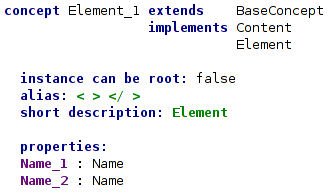
\includegraphics[scale=0.75]{./img/element_concept_common.png}
	\caption{Resulting Element{\_}1 concept}
	\label{fig:element_concept_common}
\end{figure}

Next, we are going to describe two different approaches --- the straightforward approach (section \ref{chap:straightforward_approach}) and the shortcut approach (section \ref{chap:shortcut_approach}).
The difference between these two lies in the way we create children fields for parser rules and in the way we are going to link them together using interface concepts.
Final solution will be described in section \ref{chap:structure_solution}.

\newpage

\subsection{The Straightforward Approach}
\label{chap:straightforward_approach}

The first attempt was quite straightforward and a little bit explorative, in the way that the author had to discover the MPS API that allows programmatical language generation.
Because MPS is still in development, the API isn't that well documented and some features had to be discovered through trial and error or through examination of the PE4MPS project (Section~\ref{chap:pe4mps}), which served great aid here.

\subsubsection{The Algorithm}
\label{chap:straight_algorithm}
The main idea behind the first attempt comes from the realization that when a parser rules breaks into more alternatives, we need to create a concept for each alternative.
Then we have to somehow mark them as belonging to that parser rule.
Consider the \parserrule{content} rule from our SimpleXML language:

\begin{antlr}
	\parserrule{content}    :   \lexerrule{TEXT}
           |   \parserrule{element}
           |   \parserrule{comment}
           |   \lexerrule{CDATA}
           ;
\end{antlr}

We will need to have 4 concepts that could appear anywhere the \parserrule{content} rule is referenced.
That is why we decided that for each rule with more than one alternative, we will create an interface concept.
Then for each alternative of this rule, we will create a concept that will implement this interface.
So for our \parserrule{content} example, we will get following setup:

\begin{antlr}
	\interface{IContent}   :   \concept{Content{\_}1}
           |   \concept{Content{\_}2}
           |   \concept{Content{\_}3}
           |   \concept{Content{\_}4}
\end{antlr}

Names of these concepts are derived from the name of the rule, numbers are added to alternatives correspondingly.
For rules with a single alternative, no interface is needed.
For rules that contain in-line block rules (Section~\ref{chap:subrules}), we have already created artificial parser rules in our tree representation during the parser phase (Section~\ref{chap:parsing_the_grammar}), which means we do not have to worry about them now.
\\

Now we will describe, how we linked parser rules together.
Consider the \parserrule{element} rule that is referencing the \parserrule{content} rule:

\begin{antlr}
	\parserrule{element}    :   \literal{<} \lexerrule{Name} \parserrule{attribute}* \literal{>} \parserrule{content}* \literal{</} \lexerrule{Name} \literal{>}
           |   \literal{<} \lexerrule{Name} \parserrule{attribute}* \literal{/>}
           ;
\end{antlr}

Following the algorithm mentioned above, there is one \interface{IElement} interface and two \concept{Element{\_}1}, \concept{Element{\_}2} concepts created.
For each referenced parser rule inside a concept, we create a child link and point it to the right interface.
In our example, for concept \concept{Element{\_}1}, there would be two child links pointing to \interface{IAttribute} and \interface{IContent}.
In Figure~\ref{fig:element_concept_full}, you can see the full \concept{Element{\_}1} concept.

\begin{figure}[h]
	\centering
	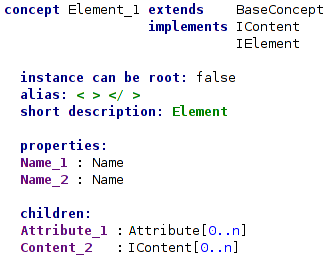
\includegraphics[scale=0.75]{./img/element_concept_full.png}
	\caption{Element{\_}1 concept's structure aspect}
	\label{fig:element_concept_full}
\end{figure}

Naming convention of child links also contains numbers, because names have to be unique.

\subsubsection{The Layer Problem}
\label{chap:layer_problem}

The algorithm mentioned above will leave us with an MPS language that follows given structure correctly and could be used to represent code in that language inside MPS correctly. Editing the code will not be possible yet, as there is no editor aspect defined so far.
There is one problem, however, concerning usability of such language.
We will demonstrate this problem on the SimpleXML language, using \parserrule{element} and \parserrule{content} rules:

\begin{antlr}
	\parserrule{content}    :   \lexerrule{TEXT}
           |   \parserrule{element}
           |   \parserrule{comment}
           |   \lexerrule{CDATA}
           ;

	\parserrule{element}    :   \literal{<} \lexerrule{Name} \parserrule{attribute}* \literal{>} \parserrule{content}* \literal{</} \lexerrule{Name} \literal{>}
           |   \literal{<} \lexerrule{Name} \parserrule{attribute}* \literal{/>}
           ;
\end{antlr}

When we would be editing code in this language, the MPS auto-complete would give us aid when filling out all properties and children of inserted concepts.
Imagine there is a freshly inserted \concept{Element{\_}1} concept (a concept representing the full XML element as is stated in the first alternative of the \parserrule{element} parser rule).
This setup can be seen in the left part of Figure~\ref{fig:layer_problem}.
Now, we would like to insert some content inside.
Let's say we would like to insert a nested XML element inside.
We would place the cursor in the content placeholder and press Ctrl+Space to view the auto-completion options.
\\

Following the algorithm mentioned above, we have created a child link of the \concept{Element{\_}1} concept of type \interface{IContent}.
There exist 4 concepts that implement the \interface{IContent} interface as per each alternative of the rule.
MPS evaluates this and gives us 4 options inside the auto-complete.
This auto-complete is captured in Figure~\ref{fig:layer_problem}.

\begin{figure}[h]
	\centering
	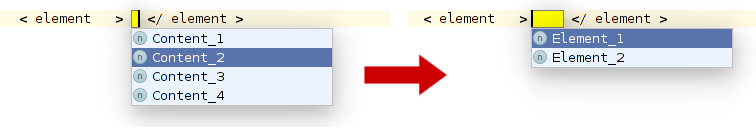
\includegraphics[width=\textwidth]{./img/layer_problem.png}
	\caption{Layer problem in auto-completion}
	\label{fig:layer_problem}
\end{figure}

In order to correctly insert another nested element inside, we would have to first insert a \concept{Content{\_}2} concept inside \concept{Element{\_}1} that has an \interface{IElement} child inside (and nothing else).
Then, as a second step, we would call for the auto-complete again and insert either \concept{Element{\_}1} or \concept{Element{\_}2} inside \concept{Content{\_}2}.
This mean that we have to go through two steps and in the first one either guess correctly (or remember the grammar rule's alternative order), to know, which item of the auto-complete we should go with.
\\

And the problem goes both ways --- if we decide to replace the nested \concept{Element{\_}1} with, let's say, an XML comment (a \concept{Comment} concept), we need to delete both intermediary layers before we get back to the original \concept{Content{\_}X} crossroads.
Meanwhile, the user cannot really see, what is happening, since the intermediary level has no appearance or indicator.
This leads to confusion on user's part.
\\

We tried to ease this situation up by creating aliases for concepts derived from their content (names such as “Element content” or “CDATA content” instead of Content{\_}N), but the problem goes beyond this.
Take into consideration that the SimpleXML grammar is a very simple one.
More sophisticated languages may have more than two intermediary layers and writing code would consist of clicking through a large number of auto-completes like shown in the example above.
There is also nothing preventing authors of grammars from naming these helper layers in a completely unrelated manner, which would make user's orientation even harder.
After all, these layers come into existence when the grammar is being written, so that it is more readable for humans and maybe better maintainable by the author.
It has nothing to do with making the AST simple for the ANTLR parser.
ANTLR is very capable and handles this probably very well in any form.
\\

Furthermore, using in-line subrule blocks makes this even a bigger problem as the block rule's names are auto-generated by our parser and differ only by numbers, even though the alias assigning process improves the situation by a bit.
But from the point of view of the grammar's author, it is an invisible layer of rules nested inside.



\subsection{The shortcut approach}
\label{chap:shortcut_approach}

After the problem with layers crossed our path in the first attempt, we took a step back and tried to reevaluate our approach.
The second attempt is based on looking at elements of alternatives (parser rule references) and asking: "which concepts could be inserted in this place?".
Consider again the \parserrule{content} rule and its child rules:

\begin{antlr}
	\parserrule{content}    :   \lexerrule{TEXT}
           |   \parserrule{element}
           |   \parserrule{comment}
           |   \lexerrule{CDATA}
           ;

	\parserrule{element}    :   \literal{<} \lexerrule{Name} \parserrule{attribute}* \literal{>} \parserrule{content}* \literal{</} \lexerrule{Name} \literal{>}
           |   \literal{<} \lexerrule{Name} \parserrule{attribute}* \literal{/>}
           ;

	\parserrule{comment}    :   \literal{<!--} \lexerrule{TEXT} \literal{-->} ;
\end{antlr}

We started building on top of the algorithm mentioned in \ref{chap:straight_algorithm}.
This leaves us again with a concept for each alternative and an interface for parser rules containing more alternatives.
We can see that the content rule can ultimately expand into following concepts:

\begin{itemize}
	\item \textbf{Content{\_}1} (TEXT)
	\item Content{\_}2 $\rightarrow$ \textbf{Element{\_}1}
	\item Content{\_}2 $\rightarrow$ \textbf{Element{\_}2}
	\item Content{\_}3 $\rightarrow$ \textbf{Comment}
	\item \textbf{Content{\_}4} (CDATA)
\end{itemize}

The layer problem (\ref{chap:layer_problem}) dwells in the need of inserting the \concept{Content{\_}2} concept before being able to insert one of the \concept{Element{\_}1} or \concept{Element{\_}2} concepts.
We would like to avoid that and offer directly the concepts that are at the end of the chain (in bold).
These are concepts we would like to see in the auto-completion menu.
They cannot transparently break into more rules and for the sake of text we will call them \textbf{end concepts}, or when talking about the grammar rule tree \textbf{end rules}. 
\\

We will describe an algorithm, that will find all end rules for a given parser rule, and later utilize it.

\subsubsection{The algorithm}
To find end rules for each parser rule, we can recursively scan through the parser tree, that we have built before. For each parser rule, we will try to find paths leading to some end rule through its alternatives:

\begin{itemize}
	\item Whenever we find an alternative, that contains only one element, and this element is a reference to another parser rule, we have found an intermediary level that can be transparently hidden from the user of the language. 
	We will continue recursively processing alternatives of this “level” rule (we are not at the end of the chain yet).

	\item Otherwise, we have found an end rule (recursion stops here).
\end{itemize}

We have expressed this algorithm using a pseudo-code:

\label{chap:shortcut_algorithm}
\begin{antlr}
	FindPathsToEndNodes(\parserrule{R}):
	1)  Define \parserrule{L} as an empty list of list of nodes
	2)  Return FindPathsToEndNodes(\parserrule{R}, \parserrule{L})
	
	FindPathsToEndNodes(\parserrule{R}, \parserrule{L}):
	3)  Define \parserrule{Q} as list of list of nodes
	4)  For each alternative \parserrule{A} of rule \parserrule{R}:
	5)      \parserrule{L1} = Clone(\parserrule{L})
	6)      If \parserrule{A} is a parser rule with only one element \parserrule{E}:
	7)          Let \parserrule{I} be interface/concept representing rule \parserrule{E}
	8)          \parserrule{L1}.Add(\parserrule{I})
	9)          \parserrule{P} = FindPathsToEndNodes(\parserrule{E}, \parserrule{L1})
	10)          \parserrule{Q} = Merge(\parserrule{Q}, \parserrule{P})
	11)      Else
	12)          \parserrule{L1}.Add(\parserrule{R})
	13)          Let \parserrule{P} be concept representing \parserrule{A}
	14)          \parserrule{L1}.Add(\parserrule{P})
	15)          \parserrule{Q}.Add(\parserrule{L1})
	16)  Return \parserrule{Q}
\end{antlr}

By appending the rule that is leading to current element (line 12) and then appending that alternative's element itself (line 14), we will get a path that contains the full path and the target end rule as the last element of the chain.
The result of this algorithm, for example for the \parserrule{content} rule, equals the listing of the five paths mentioned in the beginning of this chapter.
\\

We can do this for all parser rules and for each rule we will get a list of paths that lead from that particular rule to an end node. 
We will call these paths \textbf{shortcuts}, as they can provide a shortcut from the rule to the end of chain. 
Now that we have these, we will talk about several ways, how to use them to make our language better.

\subsubsection{Smart auto-completion}
The first attempt on how to use shortcuts (result of the algorithm in \ref{chap:shortcut_algorithm}) was built on top of the previous approach. 
There were no structural changes when it came to interfaces or linking concepts together.
We imported everything just the same and then added some more functionality.
\\

We were trying to solve the most obvious problem in front of us --- the auto-completion. 
We would like to improve it, so that it offers us only end concepts.
Luckily for us, MPS gives us the ability to create custom auto-complete menus and use those instead of the built-in one.
This means, that we are going to be able to construct our own menu containing only end nodes.
Unfortunately, it requires us to implement some non-trivial mechanisms.

\paragraph{Defining the auto-complete}

The auto-complete menu is bound to a cell of the projectional editor containing a reference to one of the children of a concept.
Let's say we are again talking about the concept that represents the element rule's first alternative.
As described above earlier in the process (\ref{fig:element_concept_full}), we created:

\begin{itemize}
	\item An interface \interface{IContent} representing four different alternatives that the content rule can break into

	\item A child of the \concept{Element{\_}1} concept, that references the \interface{IContent} rule
\end{itemize}

Somewhere in the editor aspect of the \concept{Element{\_}1} concept, there will be a cell referencing the concept interface \interface{IContent}. 
The cell, together with the auto-complete property can be seen in figure \ref{fig:autocomplete_cell}.

\begin{figure}[h]
	\centering
	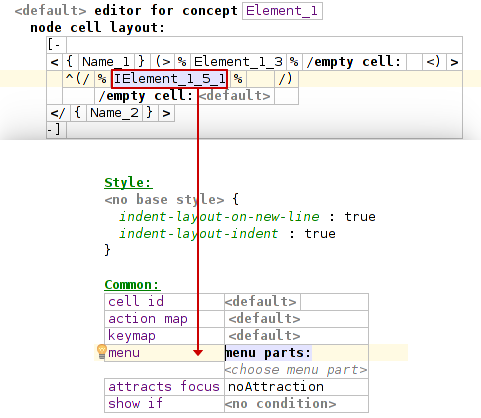
\includegraphics[width=\textwidth]{./img/autocomplete_cell.png}
	\caption{Auto-complete property \textbf{[TODO: edit image]}}
	\label{fig:autocomplete_cell}
\end{figure}

We would like to create an auto-complete for this cell, that would contain following options (end concepts):

\begin{itemize}
	\item Content{\_}1
	\item Element{\_}1
	\item Element{\_}2
	\item Comment
	\item Content{\_}4
\end{itemize}

Because we are inside MPS everything is a concept node.
In order to create an auto-complete menu, we need to create some BaseLanguage node and put it inside some AST (referencing the menu).
More precisely, we will create an instance a concept called \texttt{CellMenuPart{\_}ReplaceChild{\_}CustomActionConcept}, contained in one of many MPS's core languages.
\\

For this concept we will define a number of auto-complete options, one for each end concept, that we want to offer in the menu.
Every option has a \textbf{textual description}, \textbf{matching text} (so that we can filter through them) and most importantly a \textbf{creator method}.
If user selects that particular option, this method will be called with some contextual information in parameters and it is expected to return an instance of some concept that implements the \interface{IContent} interface.
\\

The complicated part of the process comes now, as we would like to dynamically generate the creator method.
We need to create BaseLanguage statements, that will instantiate the end concept and return it.
There is one small problem though.
Let's say the user selected the second option and decided to insert another \concept{Element{\_}1} inside.
The problem is, that \concept{Element{\_}1} doesn't implement the \interface{IContent} interface.
It only implements the \interface{IElement} interface as per the algorithm of the straightforward approach (\ref{chap:straight_algorithm}).
The shortcut, that leads to this end concept leads through the \concept{Content{\_}2} concept, that has an Element child.
This means, that we have to follow the whole path and chain individual nodes, beginning with the \concept{Content{\_}2} concept.
For this particular case it would mean to:

\begin{itemize}
	\item Create an \concept{Element{\_}1} concept and store it in a variable.

	\item Create a \concept{Content{\_}2} concept and store it in a variable.

	\item Assign the \concept{Element{\_}1} node to the right child of the \concept{Content{\_}2} node.

	\item Return \concept{Content{\_}2} node.
\end{itemize}

As we said earlier in section \ref{chap:generating_code_inside_mps}, generating BaseLanguage code is a bit more complicated because we need to either use quotation or create a large number of AST nodes. Using quotation in this case was sometimes impossible as everything is very dynamic. The finished option concept is shown in figure \ref{fig:autocomplete_action}.

\begin{figure}[h]
	\centering
	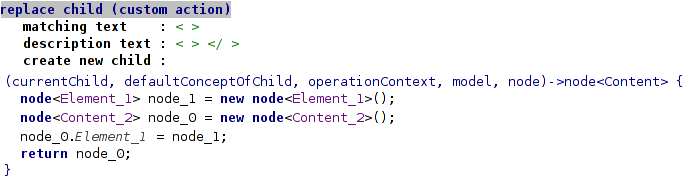
\includegraphics[width=\textwidth]{./img/autocomplete_action.png}
	\caption{Auto-complete action code (Element{\_}1 concept)}
	\label{fig:autocomplete_action}
\end{figure}

For the description text, we used concept's alias. We talk about creating aliases in chapter [TODO: alias chapter reference].
For matching text we used the shortest unique prefix of alias among all other options' aliases in given auto-complete menu.
The algorithm for searching shortest unique prefixes in a set of strings is not important from our thesis' point of view, so we decided to not go into further detail.

\paragraph{The layer problem again [TODO]}

After we implemented the auto-complete menu, coding in the imported language started to be very reasonable and comfortable since we eradicated intermediate layers. Or did we? When producing code, the language really does what one would expect, however when user starts deleting things, the layer problem occurs once more.
\\

What happens here is that when we select the auto-complete option, several layers of concept might get created and inserted into the cell. Imagine we just inserted the \concept{Element{\_}1} node. According to the creator method, this new node is wrapped inside of the \concept{Content{\_}2} node. Now let's say user changed his mind and wants to replace this XML element with a comment. He would press backspace, the XML element would disappear as expected. Then user would invoke the auto-complete menu again and expect again to have all five options at hand. What happened instead is that the \concept{Element{\_}1} node got deleted, but the wrapping \concept{Content{\_}2} one remained. The \concept{Content{\_}2} concept has only one child of type Element and that is why user only sees \concept{Element{\_}1} and \concept{Element{\_}2} as options in the auto-complete.

\paragraph {The deletion context}

Solution to this resurrected layer problem lies in controlling the deletion event. Once again, MPS' authors have equipped us with tools for doing this. We are able to specify our own handler for the deletion event for any cell of the projectional editor. But what will it look like?
\\

When deleting a node, we would like to remove the shortcut, the whole path, and effectively reversing the effect of the creator method. We decided that it will be the easiest to store the length of the path that is leading to certain node with the node. So when we are creating the node path in the creator method, we tell each node how deep or far on the path it is. In order to do this, we created a \concept{BaseConcept}, a parent abstract concept from which we will inherit all other concepts. This abstract concept will define a special integer property that will hold our information and effectively making all other concepts inherit it too. We called this property \textit{{\_}{\_}DeleteContext} and enhanced the creator method as shown in figure \ref{fig:autocomplete_action_delete_context}.

\begin{figure}[h]
	\centering
	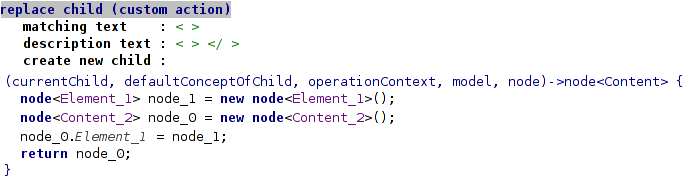
\includegraphics[width=\textwidth]{./img/autocomplete_action_delete_context.png}
	\caption{Auto-complete action extended with deletion context}
	\label{fig:autocomplete_action_delete_context}
\end{figure}

The last thing remaining is creating the backspace action. Apart from some problems with referencing the \textit{{\_}{\_}DeleteContext} property, which must be reached through the abstract \concept{BaseConcept} type, it is quite straightforward to generate a BaseLanguage code like shown below (figure \ref{fig:backspace_action}).

\begin{figure}[h]
	\centering
	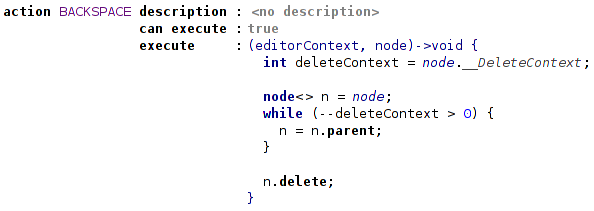
\includegraphics[width=\textwidth]{./img/backspace_action.png}
	\caption{Backspace action implementation}
	\label{fig:backspace_action}
\end{figure}

We must not forget to pin this handler to every cell that we pin the auto-complete to. After we had done this, the layer problem has finally been eradicated. The language became a bit more usable once more.

\subsubsection{Smart interfaces}

After we have implemented the smart autocomplete, we realized that there might be another way to accomplish almost the same result. It would mean changing the first step concerning concept interfaces creation.
\\

The main idea behind this is the realization that if for each concept interface there exists a finite set of end concepts, we could just create a special interface and let all these and only these end concepts implement it. It is important that other non-end concepts that are in the shortcut will not implement it, because that would put us right back where we started with the straightforward approach \ref{chap:straightforward_approach} and the layer problem \ref{chap:layer_problem}. To give an example regarding our content rule, we would create an \interface{IContent} interface concept and only following concepts would implement it:

\begin{itemize}
	\setlength\itemsep{0pt}
	\item Content{\_}1
	\item Element{\_}1
	\item Element{\_}2
	\item Comment
	\item Content{\_}4
\end{itemize}

Concepts would of course implement as many interfaces as many shortcuts lead to them. The difference is that the intermediary layers will not, preventing the layering.
\\

We still need to find end concepts for each rule, so we will keep the same algorithm for finding shortcuts as before. We, however, do not need to implement our own auto-completion (and subsequently with it no deletion handlers), because the built in default auto-completion will start to behave exactly the same way our smart auto-completion did.

\paragraph{Cardinality restriction}

So far it looks like the last approach is superior to the auto-completion one. It avoids complicated code generation and even resulting MPS languages are more simple, perhaps better performant as they are not bloated with auto-completion code. There is one small drawback though, that makes this solution suboptimal.
\\

To remind the reader --- the cardinality of an element is telling us, how many of each specific child rules can occur inside an alternative. Inside the grammar this was expressed using quantification operators (\textbf{*},\textbf{+} and \textbf{?}). The problem that appears here can be shown using these example rules:

\begin{antlr}
\parserrule{content}      :   \parserrule{element}+
             |   \parserrule{comment}*
             |   \lexerrule{CDATA}?
             ;
\end{antlr}

Notice, how we changed the cardinality of elements inside the \parserrule{content} rule. This small change will prevent us from creating a shortcut leading through this rule. We are trying to say that shortcuts that can be used for the smart interfaces approach can only lead through rules, that have cardinality [1..1] (so through an alternative with a single child element, that is a reference to a parser rule AND has this cardinality). Speaking in terms of the shortcut algorithm \ref{chap:shortcut_algorithm}, we would alter line number 6 and add this restriction to the condition.
\\

This restriction is caused by the fact that we would be unable to control children cardinality. Imagine that some alternative of some other rule contains reference to this altered \parserrule{content} rule (regardless of its quantitative operator). That means that we need to create a child holding the \interface{IContent} and setting this cardinality. But each alternative of the altered content rule requires different number of children to be inserted. Since there are no intermediary levels of nodes that could influence this, the end concept node that would be inserted in that child would inherit the cardinality of the child regardless of what the shortcut path looks like.
\\

A small example might demonstrate this better. We have an \interface{IContent} [1..1] child. If we disregarded the cardinality restriction, we could ultimately put there \concept{Element{\_}1} end concept node. But the content rule says, there can be [1..n] elements. We are still bound to insert only one though.


\subsection{Our Solution}
\label{chap:structure_solution}

In the end, we have decided to go with the shortcut approach using smart interfaces.
As we have stated above, it has several advantages, concerning the solution complexity, compared to the smart auto-completion.
It only has one disadvantage regarding the cardinality restriction, described in \ref{chap:cardinality_restriction}.
We have analyzed several ANTLR grammars (such as the JavaScript~\cite{javascript}) and we haven't found a single intermediate rule, that would be suffering from this restriction.
It is quite understandable if you think about how grammars are written.
Usually, you create the basic structure (i.e. different kinds of statements) in the simplest way possible and put the quantitative operator rather to an alternative that is referencing the structure.
\\

Based on these observations and some grammar analysis, we concluded that advantages prevail and used the last mentioned approach.

\subsection{The Structure Aspect and Other ANTLRv4 Features}
\label{chap:antlr_features}

The ANTLR grammar notation offers more features than just rule definition.
We haven't mentioned these earlier because we were focusing solely on the structure of the language.
We will mention some features and explain why we have ignored them and why they don't matter to us.
We will not spend a lot of time on describing details of these as they are well documented in the official ANTLR reference~\cite{ANTLR4reference}.

\subsubsection{Modes}

For example, just like any other parser/lexer, ANTLR gives us the possibility to switch the parsing context.
We are able to create various user-specified modes and then enter these modes when certain rules/tokens are encountered.
For each mode, we can define a different set of rules/tokens that can only be applied when the parser is in that particular mode.
The syntax is following:

\begin{antlr}
	\textcolor{gray}{// Enter mode when tag opened}
	\lexerrule{OPEN}        :   \literal{<}       -> pushMode(INSIDE) ;

	mode INSIDE;
	\textcolor{gray}{// Special rules bound to specific mode}
	\lexerrule{S}           :   \regex{[ {\textbackslash}t{\textbackslash}r{\textbackslash}n]} -> skip ;

	\textcolor{gray}{// Leave the mode when tag closed}
	\lexerrule{CLOSE}       :   \literal{>}       -> popMode ;
	\lexerrule{SLASH{\_}CLOSE} :   \literal{/>}      -> popMode ;
\end{antlr}

We didn't pay any extra attention to modes while dealing with the structural aspect because they don't really influence contents of individual concepts.
It is even possible to define concepts that control mode switching and then not including them inside any parser rule.
They still get recognized by the lexer and mode is changed.
\\

The reason that this goes beyond our interest here is partially caused by the fact, that modes are used on runtime when we are parsing actual code, whereas language structure is more of a static matter.
The only time we care about modes is when generating the TextGen aspect, and we will get back to it later in Chapter \ref{chap:textgen}.

\subsubsection{Actions, Attributes and Semantic Predicates}

Actions allow us to append code to rules and this code is then executed every time the parser applies this rule.
The code is written in the target language that you are creating the parser for.
It is then copied as a string and inserted into the method that is bound to parsing this rule.
Again, this is of a little interest to us.
Usually, this is used when creating some specific parsers for some particular scenario.
We, however, are expecting to parse general purpose languages that contain actions just rarely.
And even when they did, we cannot be sure what language will it be in and how to use it.
\\

Attributes allow us to extend some basic predefined set of properties of each rule.
We can store some arbitrary information there and later access it for example inside actions using special syntax.
From exactly the same reasons as with actions, attributes are of no interest to us.
\\

Semantic predicates tell the parser on runtime, which rules can be applied depending on specified constraints.
This is also a runtime matter.


%\pagebreak

%\section{The Editor Aspect}
\label{chap:editor_aspect}

After we have imported all concepts, their contents (properties) and linked them together (child links), it is time to define, what is the visual representation of these concepts.
Without this, we are not able to start using the language inside MPS.
\\

As stated before (Section~\ref{chap:about_editor_aspect}), MPS uses a cellular system, that allows placing concept's properties and children into a table-like arrangement.
MPS has a lot of different types of cells, that we can use:

\begin{itemize}
	\item Cells for storing values of properties -- the user can enter text inside, which is validated using the type of the property (think XML tag name).

	\item Cells for storing child concepts -- here we can store other parser rule references and build the AST further.

	\item Cells that have static fixed content, such as constant keyword -- we will use these to display literal elements.

	\item Cells that influence the layout, such as indenting.
\end{itemize}

Our import plugin has to create these cells and ideally project all of the concept's elements in there.
\\

A part of this thesis' mission was to explore, whether we can also bring some more value into this import step.
The problem with grammars is, that it serves us no aid when it comes to element layout.
The grammar only defines, what the rule breaks up into and which elements (rule references, literals..) are contained inside of each alternative.
Since the layout information is missing, we have only two options, how to tackle this problem:

\begin{itemize}
	\item Get this information from the user by prompting for it somehow.
	\item Keep everything automatized and generate the information using some heuristic.
\end{itemize}

It is a very hard problem, though since our plugin doesn't really understand the contents of the grammar on some higher level.

\subsection{The Interactive Approach}

Since the layout information is just missing, we decided to ask the user for it.
The first idea on how to tackle this problem was to interactively prompt the user during the import process.
We would somehow select rules, that we consider important, and give the user several visual options on how we think this rule might be laid out.
The user would pick one and we would use this information to create the editor aspect.
There are some problems with this, though, that led to rejecting this approach.

\subsubsection{Detecting Interesting Rules}

Firstly, we would have to be able to tell, which rules might be worth "discussing" with the user.
\\

The first idea for a heuristic indicating these "interesting" rules was based on a number of elements contained in rule's alternative.
For simple rules, which there usually is a big number present in the grammar, we would skip them.
For complex rules (let's say 5 elements and more), we would ask the user for help with the layout.
The heuristic isn't bad, it would detect complicated rules, such as cycles, branching commands and so on, so it might be a sufficient, yet simple, solution.
It, however, has some problems --- rules describing a block of statements are usually very simple, example given being the JavaScript one:

\begin{antlr}
	\parserrule{statementList} : \parserrule{statement}* ;
\end{antlr}

This rule would be skipped by our heuristics since the alternative has only one element, but in most general purpose languages, this is exactly the kind of statement, that we would like to adjust, since normally we put each statement on a separate line.
There are dozens of rules, that have this form (method parameters, operands, ...), and we have no means of recognizing, that this particular one should be a vertical list (meaning its elements should be separated by a new line).
\\

Another heuristic suggestion was detecting pair symbols among alternative's literal elements.
Usually, characters such as braces are a good indicator of some indenting.
We, however, did not implement any of these heuristics, because, in the end, we decided to abandon the interactive approach completely, as described below in Section~\ref{chap:interactive_approach_evaluation}.
That is why we will not go into more detail here.

\subsubsection{Fixing Rule Layout}

Once we have detected a rule, that might have some interesting layout, we would ask the user to help us with adjusting it.
Consider, for example, the first alternative of the \parserrule{element} rule from the XML language:

\begin{antlr}
	\parserrule{element}  :   \literal{<} \lexerrule{Name} \parserrule{attribute}* \literal{>} \parserrule{content}* \literal{</} \lexerrule{Name} \literal{>} ;
\end{antlr}

Let's say, we would prepare few versions of how we think the layout could look like.
We would present these options to the user and let them choose.
We could ask the user, whether attributes should be spread out horizontally or each on a new line.
We could and probably would have to do this for each element since the plugin has no real understanding of the content.
We would have to ask for indentation, line breaks etc. because if we were to guess, we would probably guess wrong since there are just too many options.
The user would probably end up finalizing the layout himself.
\\

The other option could be in form of some sophisticated smart dialog, where the user would control the layout by dragging the elements around or position them through some text field.
This would be probably better, but we would be reimplementing already existing functionality, that is already present inside MPS.
Again, we are not going into any more detail here, as this approach was rejected because of reasons mentioned below.

\subsubsection{Approach Evaluation}
\label{chap:interactive_approach_evaluation}

The author of this thesis came to a conclusion, that the results of the interactive approach would be most likely quite suboptimal.
It would be hard to recognize rules, that are in need of a refactoring.
Furthermore, when asking for user's help, we would just duplicate the functionality of MPS's built-in projectional editor.
We would hardly mimic all of its functionality and put a lot of effort into something already existent.
Moreover, our end user is expected to have knowledge of the MPS editor, since he is importing language there.
This means, that he probably knows his way around the projectional editor too.
It wouldn't make sense to force the user to learn to work with our own interactive dialog, while in the background, this dialog would be just translating the layout back into the terms of the projectional editor.
Implementing such mechanism would also probably be very complicated.
\\

To put it a bit differently --- we wouldn't be sparing the user from any manual work, we would be only changing the environment, where this work happens.
We would be shifting it from the MPS projectional editor designer into our interactive dialog.
We would be shifting it from a fully featured MPS environment, the user probably already knows, into a feature-wise way poorer environment, the user sees for the first time.
We would be doing this shift for a price of reimplementing already existing mechanisms.
We would also need to decide, where to draw a line and which layout features we will cover in our interactive dialog (say line breaks and indenting) and which features we would leave out (code colouring, spacing..).
If we didn't draw this line, we would end up reimplementing the whole MPS projectional editor designer.
Furthermore, for every feature, that we would choose to include, we would have to implement special behaviour inside the interactive dialog and then another logic that would translate settings from this dialog into the editor aspect.
And even if we accomplished everything mentioned above, we still believe (and have confirmed that by experimenting), that the language would still need to be adjusted inside the projectional editor designer.
\\

From reasons stated above, we rejected the interactive approach.
From exactly the same reasons, we concluded, that any approach, that would require user input, would be suboptimal to just leaving the user adjusting the layout inside the MPS editor designer.

\subsection{The Learning Approach}
\label{chap:learning_approach}

Since we have rejected user-input based approaches, we are left with heuristics.
The second approach is more complex and might yield better results.
We have, however, not implemented it to a stage, that would be presentable, as we met some obstacles.
We would like to describe it anyway, so possible follow-up work might take it into consideration.
\\

\subsubsection{Approach Principle}

The learning approach would require the user to, together with the grammar file, supply a set of valid source files written in the imported language.

\begin{enumerate}
	\item The plugin would automatically generate an ANTLR parser for this language using the ANTLR library, which provides this functionality.

	\item It would alter the code of the generated parser and add some additional functionality, described below.

	\item It would compile the parser into an executable form.

	\item It would use the parser to parse the supplied source code and extract information about the layout of the code.
\end{enumerate}

The benefit of this approach is, that the imported language would inherit its code style from the user, as it would learn directly from his code.
The quality of the extracted information would depend on the amount of the code supplied.
So far, this approach sounds very complicated --- extracting layout information sounds like a difficult problem on its own.
We have, however, found a simple way, how to mine information very efficiently.
\\

When the ANTLR parser is parsing the code, in its first stage, it reads the input and tries to split it into tokens.
In the second stage, it tries to map the token stream onto parser rules of the language and build an AST.
Earlier, in step 2, we said, that we would change the code of the parser.
We would make sure, that each parsed token would remember additional information --- the number of the line it appeared on.
This is an easily accessible property of the parser and the ANTLR framework gives us a lot of room for an adjustment like this.
\\

\noindent
For example, for our \parserrule{element} rule

\begin{antlr}
	\parserrule{element}  :   \literal{<} \lexerrule{Name} \parserrule{attribute}* \literal{>} \parserrule{content}* \literal{</} \lexerrule{Name} \literal{>} ;
\end{antlr}

\noindent
and following source code,

\begin{antlr}
	1   <div>
	2      ... some content ...
	3   </div>
\end{antlr}

\noindent
it would yield something like this:

\begin{antlr}
	TOKEN LINE
	----------
	<       1
	Name    1
	>       1
	\textcolor{gray}{...}
	\textcolor{gray}{// Here, tokens of the content would come}
	\textcolor{gray}{...}
	</      3
	Name    3
	>       3
\end{antlr}

From this, we could clearly derive, that there is a line break between the first closing \textit{greater-than} bracket, the content and then again when the closing tag starts.
Probably, we might also be able to detect indentation, if we would decide to store the column information too, but we haven't explored this possibility.

\subsubsection{Approach Evaluation}

We have started implementing a proof of concept for this approach, so that we can see, whether it is a viable solution.
Unfortunately, there were some obstacles, due to which we haven't finished the implementation.
The biggest problem, that we have identified, was parser generation.
We found out, that even a small tweaks in the grammar, that the user might perform in order to improve the resulting MPS language, can break it enough so that the automatically generated ANTLR parser is not parsing the code correctly.
We talk further about this problem in more detail in Chapter~\ref{chap:breaking_the_parser}.
\\

Other problems, that we have identified, were connected to the environment, where it might not be always possible, to perform actions such as parser generation, parser compilation or dynamic loading of the parser.
More problems concerned the algorithm itself, where we would need to be able to match language concepts with all tokens that belong to it.
Mapping the parsed ANTLR AST to the MPS one is a complex problem, that is also connected to parsing any given text source code and importing it inside MPS.
This is considered as an advanced functionality, that will probably be subject to a separate follow-up work.
\\

Because of the overall complexity of this approach and because of reasons stated in Section~\ref{chap:editor_solution}, we have decided to abandon the implementation and only suggest it as a possible follow-up.
We, however, concluded, that this might be a viable solution for detecting code layout.

\subsection{Our Solution}
\label{chap:editor_solution}

When the author of this thesis worked on the plugin, he noticed, that the most tiresome and likely error-prone part of working on the editor aspect is incorporating all concept's properties, children, and constant fields into the editor.
This means a manual creation of all cells, that should appear in the visual representation.
We identified this phase as a time consuming but also quite straightforward, as it does not require any major thought on user's part.
We have also further noticed, that when the plugin would do this heavy lifting, even without layout detection, further adjustments of the editor are very fast since MPS enables doing this very efficiently.
We noticed, that even the most obvious way of editor generation, such as plain inlining of all of the cells in a single row (shown in Figure~\ref{fig:editor_adjustment} on top), might be a sufficient solution.
In Figure~\ref{fig:editor_adjustment}, we can see an editor adjustment of the \concept{Element{\_}1} concept, that can be done in just a few clicks, but finalizes the editor to its perfect form, better than any heuristics would come up with.
\\

\begin{figure}[h]
	\centering
	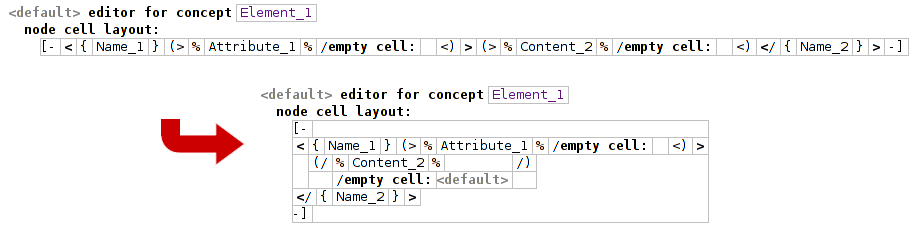
\includegraphics[width=\textwidth]{./img/editor_adjustment.png}
	\caption{Projectional editor adjustment of the Element{\_}1 concept}
	\label{fig:editor_adjustment}
\end{figure}

From these reasons, we concluded, that for our cause, it might be sufficient, if the plugin only prepared contents of all editor aspects and the end user would take it from there, reaching optimal results in a very short time.
We have confirmed this assumption by importing the JavaScript language~\cite{javascript} and manually adjusting all editors, that needed it, in a less than hour time.
We have described this further in Chapter~\ref{chap:examples}.
Further improvements might be a subject for a follow-up work, potentially leveraging the second approach, we have described above in Section~\ref{chap:learning_approach}.



\pagebreak

\section{The TextGen Aspect}
\label{chap:textgen}

TextGen aspect's purpose is telling each concept, what the real text code generated out of it will be, once we want to turn our MPS code into a real program.
Basically, it's a single method definition for each concept of the language.
This method has several parameters, such as the currently processed node and some contextual information.
It is, however, not returning a string as perhaps expected, but rather manipulates an output buffer/stream using some built-in functions.
When generating the code of a program, MPS calls this method for the root concept of the program.
It is up to this concept's TextGen method to append its children into the stream by invoking their TextGen methods subsequently.

\subsection{Our Goal}

What we would like to do here, is to create a TextGen aspect for each concept and generate some BaseLanguage code for its TextGen method.
The TextGen method is, again, an AST built out of concept nodes as described in section \ref{chap:generating_code_inside_mps}.
We need to create a root node of the method and to its body child add a list of BaseLanguage statement nodes that represent the code of the method.
Let's illustrate this using our SimpleXML example, namely the \concept{Element{\_}1} concept, that represents the full XML tag with content and is given by the first alternative of the \parserrule{element} rule:

\begin{antlr}
	\parserrule{element}   :   \literal{<} \lexerrule{Name} \parserrule{attribute}* \literal{>} \parserrule{content}* \literal{</} \lexerrule{Name} \literal{>}
          \textcolor{gray}{|   \ap<\ap Name attribute* \ap/>\ap}
          \textcolor{gray}{;}
\end{antlr}

A very basic example of a BaseLanguage code, that we would like to generate for this concept, is shown in Figure \ref{fig:textgen_example}.

\begin{figure}[h]
	\centering
	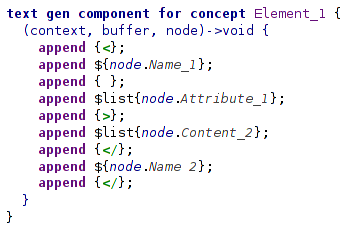
\includegraphics[width=90mm]{./img/textgen_example.png}
	\caption{Example of a TextGen aspect}
	\label{fig:textgen_example}
\end{figure}

We can see that we gradually append all literals, properties, and children in the same order as they appear in the grammar definition.
This part of the process holds no first-hand complications.
We still need to generate BaseLanguage code dynamically, which in some cases might be a challenge.
We figured how to overcome those challenges earlier in Section~\ref{chap:generating_code_inside_mps}.
There are, however, some hidden problems along the path.

\subsection{Whitespaces}
\label{chap:whitespaces}

As you might have noticed, there was no whitespace handling inside of our SimpleXML grammar.
For example in the \parserrule{element} rule, there is \lexerrule{Name} the element directly followed by \parserrule{attribute}*, but in the XML language we require at least one space as a separator.
So how does the parser know how to split tokens, how many whitespace characters are expected, and which characters are whitespace in the first place?

\begin{itemize}
	\item How does our TextGen generator know, that there should be a space in between \parserrule{attribute} and \lexerrule{Name} but is not required between \literal{\textless} and \lexerrule{Name}?

	\item How does it know there is no space between quotes and an attribute value inside the \parserrule{attribute} rule?

	\item And how about multiple attributes --- do they need to be separated by spaces?
\end{itemize}

\subsubsection{Whitespace Handling in ANTLR}

We have left the whitespace handling part out earlier in order to keep things more simple as we were paying attention to the structure of the language in the first place.
There are two ways, how we can deal with whitespaces in ANTLR:

\begin{itemize}
	\item We can define special tokens, that don't need to be used inside any parser rule.
	We mark them with special flag, telling the parser to skip these characters when this token is matched:

	\begin{antlr}
		\lexerrule{WHITESPACE}   :  \regex{[ {\textbackslash}r{\textbackslash}n{\textbackslash}t]+}   -> skip;
	\end{antlr}

	\item The second possibility is to create a similar rule to the one above, but leaving out the skip flag.
	Then, we explicitly reference this token in every parser rule, where whitespace can occur.
	This sometimes means hundreds of different positions, so it is generally not a recommended approach.
	There are however cases, where this is inevitable due to the nature of the ANTLR lexer.
\end{itemize}

\subsubsection{The Whitespace Problem}

The problem, that arises here, is that the skip syntax hides the whitespace information from the grammar.
We have no way of tracing this information back.
If, on the other hand, we decided to go with the explicit definition, and put \lexerrule{WHITESPACE} tokens everywhere, we would encounter much bigger problem.
From the point of view of the TextGen aspect, it would help us a bit, but not completely, as we still don't know what string represents the rule.
Secondly, when creating the structural aspect, we would create a property for each of these token references as per Section~\ref{chap:common_ground}.
The effect of that would be, that the imported MPS language will become unusable.
The code will be full of placeholders waiting for whitespace characters (even though they might be unnecessary, i.e. [0..n]).
\\

We could try harder and ask the user himself, whether there are any whitespace detecting rules or try detecting them ourselves.
But even this will not solve the problem, as the whitespace can be easily entangled inside non-whitespace tokens as shown below with the \parserrule{chardata} rule.
\\

If we look into existing ANTLR grammars, we can see that things get even more complicated.
ANTLR, just like as any other parser/lexer, gives us the possibility to switch the parsing context.
We are able to enter any user specified mode and then apply a different set of rules depending on current mode, which gives us more flexibility.
This means we can handle whitespace both implicitly and explicitly at the same time inside one grammar based on the mode.
Secondly, there is the possibility of capturing whitespace together with other characters.
Consider the following excerpt from the official ANTLR XML grammar:

\begin{antlr}
	\parserrule{element}     :   \literal{<} \lexerrule{Name} \parserrule{attribute}* \literal{>} \parserrule{content}* \literal{</} \lexerrule{Name} \literal{>}
	            |   \literal{<} \lexerrule{Name} \parserrule{attribute}* \literal{/>}
	            ;

	\parserrule{content}     :   \parserrule{chardata}?
                ((\parserrule{element}? | \lexerrule{CDATA} | \lexerrule{COMMENT}) \parserrule{chardata}?)* ;

	\parserrule{chardata}    :   \lexerrule{TEXT} | \lexerrule{SEA{\_}WS} ;

	\lexerrule{TEXT}        :   \regex{~[<&]+} ;

	\lexerrule{SEA{\_}WS}      :   (\literal{ }|\literal{{\textbackslash}t}|\literal{{\textbackslash}r}? \literal{{\textbackslash}n})+ ;

	\lexerrule{OPEN}        :   \literal{<}             -> pushMode(INSIDE) ;

	mode INSIDE;
	\lexerrule{S}           :   \regex{[ {\textbackslash}t{\textbackslash}r{\textbackslash}n]}       -> skip ;
	\lexerrule{CLOSE}       :   \literal{<}             -> popMode ;
	\lexerrule{SLASH{\_}CLOSE} :   \literal{/>}            -> popMode ;
\end{antlr}

What is happening here, is that the author decided to skip whitespace characters only when we are inside of XML tags (see that the \parserrule{element} contains no explicit whitespace tokens).
On the outside, they are being cleverly swallowed by the \parserrule{chardata} rule (its second alternative), that wraps any content.
The \parserrule{content} rule is written a bit differently from our SimpleXML version.
It is a little bit more complicated, but the shorter structure, showing all the different ways we can express the grammar in.
\\

The problem we find here is, that with all the features ANTLR has to offer, there are just too many ways, how we can handle whitespaces and they can get all mixed up together just like the previous example showed.
In the worst scenario, from the TextGen point of view, the language is skipping all whitespace characters silently and thus removing the information from the grammar completely.
\\

This leaves us with the original question and the root problem --- \textbf{how does our TextGen aspect know between which children there must be a whitespace and where it is forbidden so that the produced code is a valid one?}

\subsubsection{Possible Improvements}

Following up on the question posed in the previous paragraph, we can ask ourselves a different question.
If not our TextGen, how does the ANTLR parser know where whitespaces are due?
Surely the parser must know, otherwise, it wouldn't be able to tell wrong code from the right.
Well, the answer is, that it knows once it starts parsing some code depending on the inner state of the parser.
Context modes make this quite simple.
They are quite easy to work with on runtime when we are actually parsing some source code, but it is impossible to determine the mode for rules statically.
In other words, it is impossible to detect, whether we are swallowing whitespaces silently for given rule or not.
This is caused by the possibility to jump between modes in almost any manner and therefore use one parser rule in different contexts.
\\

We do not, however, necessarily need to put different amounts of different whitespace characters in random places.
We only need to find places, where we are sure they must be at in order to make the code valid.
Then, we can put a single space there.
Generally, it doesn't have to be a space character, but since we are aiming for general purpose languages, we will go with the very frequently used space character.
We could get some hints from the way the lexer is splitting source code into tokens, which is happening practically statically too.
Consider the following setup:

\begin{antlr}
	\parserrule{element}    :   \literal{<} \lexerrule{Name} \parserrule{attribute}* \literal{>} \parserrule{content}* \literal{</} \lexerrule{Name} \literal{>} ;

	\parserrule{attribute}  :   \lexerrule{Name} \literal{="} \lexerrule{TEXT} \literal{"} ;

	\lexerrule{Name}       :   \regex{[:a-zA-Z]([:a-zA-Z]|-|{\_}|\textbackslash.|[0-9])*} ;

	\lexerrule{TEXT}       :   \regex{~[<"]*} ;
\end{antlr}

From the general knowledge of XML, we know that there is no space needed between the opening bracket of an XML tag and the name of the tag (i.e. \textbf{{\textless}img}).
On the other hand, there has to be one between the name of the tag and the name of the first attribute (i.e. \textbf{{\textless}img src=...}).
But why is that?
Simply, because the lexer needs to parse the input source into tokens using available lexer rules (regular expressions).
If it encounters a whitespace, it will stop parsing previous token (unless there is space allowed in it), parse the whitespace one (throw it away when skipping) and continue with the next one.
\\

The reason the parser cannot differentiate tag name from attribute name without a separator is caused by their regular expressions.
Consider a string \textbf{A}, representing the tag name (a string, that can be matched by the regular expression of the \lexerrule{Name} rule).
Let string \textbf{B} be a string representing the attribute name.
Whenever \textbf{A} and \textbf{B} share some same characters, we cannot clearly state, where one ends and the other starts (when placed together).
More precisely, \textbf{A} can end with same characters as \textbf{B} can start with.
Even more precisely, some suffix of \textbf{A} can be some prefix of \textbf{B}.
In our case they are coincidently both given by the \lexerrule{Name} rule, but in general case we really care about any possible substrings.
\\

Determining whether a suffix of a string matched by one regular expression can be a prefix of a string matched by a different regular expression is not an easy task.
We could try to generate strings that satisfy both regular expressions, but probably the only complete solution to this problem would be to construct automata representing both expressions.
Then we would need to examine them somehow, in order to detect similarity.
\\

Now what happens, if one of our children, that can have zero cardinality, is empty (no element attributes)?
What are we going to do about whitespaces wrapping this child?
In this case we should probably do the same suffix/prefix comparison with the next-next child on the way, skipping the empty one.
Additionally let's not forget that all this logic needs to be contained in generated BaseLanguage code.
\\

We have decided to settle for a more simple heuristics, which is described in section \ref{chap:textgen_solution}.

\subsection{Layout}

We have already established, that whitespaces are hard to get right.
But how about the code layout itself?
What if we want to produce more readable code by adding i.e. indentation or line breaks?
Can we for example use the same information, we were mining when building the projectional editor?
It would seem like the editor and code layout are very close to each other and since we were unable to resolve editor problems fully (\ref{chap:editor_aspect}), we won't be able to leverage the information here neither.

\subsubsection{Universal TextGen}
One idea, on how to approach layout inside the TextGen aspect, would be creating a really smart universal TextGen method.
It would be static (always the same, independently of the grammar) and it would be the same for each concept of the language.
It could read the projectional editor definition and then somehow try to mimic this layout on output.
This might be quite straightforward, because each cell has its specific function, that could be translated into a text layout.
The added value of this approach would be, that whenever user decides to adjust and improve the projectional editor, it would get automatically reflected inside this universal TextGen.
It would also have a drawback, that when user would want to change the TextGen definition for some concept, he would have to build it from scratch.
\\

After this proposal was discussed with JetBrains, it was immediately rejected.
The main reason for this being, that aspects should be independent of each other.
This means, that when someone would like to introduce an extension of a language and change the editor, it might influence the TextGen in a way that, it would start generating invalid code (e.g. we could for example easily remove the “if” keyword from the projectional part).
Sometimes we might also want to define more projectional editors and switch between them, which would also make this dysfunctional.
This is probably the reason that JetBrains haven't introduced their own universal TextGen so far (just like they introduced a default projectional editor).

\subsection{Our Solution}
\label{chap:textgen_solution}

After the analysis, we have come to a conclusion, that the problem of TextGen layout is quite similar to the one we have seen with the projectional editor, described in chapter \ref{chap:editor_aspect}.
Since we are mostly dealing with text-based languages, their editor representation must be almost the same as their expected text output.
Once we would have some information about the layout for generating better projectional editor, we could leverage the same information and use it for TextGen improvement too.
We have, however, decided, that adjusting the editor manually, after the import is done, is for now the fastest and the most efficient way how to deal with this problem, so we have no information to leverage here.
\\

Adjusting the layout, speaking in the terms of TextGen, means adding line breaks and indentation --- practically the same as what we are doing with the editor aspect.
Nonetheless, aside from layout, there is still the problem concerning whitespaces, that we described above in \ref{chap:whitespaces}.
We decided not to go into full depth and solve the problem using regular expression automata.
We have, however, tried to improve the situation using some really simple heuristics which gave surprisingly good results.
\\

We have started with a very basic TextGen, that would insert spaces in between every two elements of the concept.
Then we started restricting spaces on positions where we thought they are not needed.

\begin{enumerate}
	\item We have concluded, that whenever there is a literal, it is a plain string token defined in the grammar, that might, in most cases, get recognized by the parser safely without the need for a whitespace separator around (think \textbf{'\textless'} in XML).
	So whenever there is a non-alphabetical literal, we omit spaces around it.

	\item Next, we were looking at properties (non-literal, but regex lexer rules).
	These are strings inserted by the user of the language, whose form is constrained by a regular expression (think XML tag's name).
	If these are neighboring a literal rule, we look at that literal rule's content.
	We expect that the user will be inputting some alphabetical content (variable/method/class names, identificators, etc.).
	If the neighboring literal rule ends with an alphabetical character, we insert space, otherwise, we omit it.
	This will help in cases such as insides of quotes, next to semicolons or around brackets, but on the other hand, it will separate usual language keywords (function, var, in, etc.) from other content.

	\item We check for element emptiness (child not present) and do not insert spaces when elements are empty so that spaces do not accumulate.

	\item When two children concepts are next to each other, we always insert space.

	\item Sequences of children are separated with space.
	This is the place where we might later want to manually substitute it with a line break.
	Think repeating \parserrule{content} inside an XML tag or list of XML attributes.
\end{enumerate}

These few simple heuristics have left us with some very nice results (tested mostly on XML, JSON, and JavaScript). Figure \ref{fig:textgen_final} shows an example of a TextGen aspect for the full SimpleXML element.
\\

\begin{figure}[h]
	\centering
	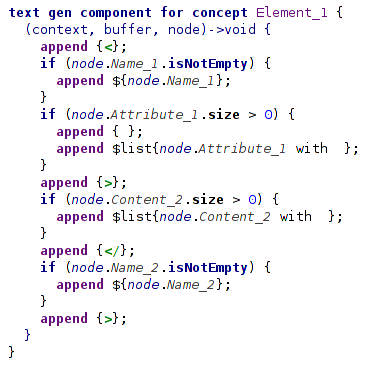
\includegraphics[width=95mm]{./img/textgen_final.png}
	\caption{Generated TextGen aspect for the SimpleXML element}
	\label{fig:textgen_final}
\end{figure}

If we wanted to manually adjust this generated code, so it generates nice indented XML code, we only need to wrap the \concept{Content{\_}2} child with indentation and change the sequence separator to a new line character.
This is a very fast and small adjustment, so we concluded that it is right to expect the user to do this kind of adjustments on his own.
Resulting adjusted aspect is shown below in Figure \ref{fig:textgen_adjusted}.

% TODO: zarovnat nahoru
\begin{figure}[!ht]
	\centering
	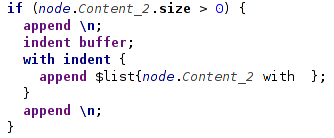
\includegraphics[width=85mm]{./img/textgen_adjusted.png}
	\caption{Adjusted indentation inside the TextGen aspect}
	\label{fig:textgen_adjusted}
\end{figure}